\section{量子傅立叶变换(QFT)}
首先, 考虑一个$2^n$维数组$\{x_j\}$($j=0, \cdots, 2^n-1$), 他的离散傅立叶变换$\{y_k\}$($k=0, \cdots, 2^n-1$)为:

\begin{equation}
	y_k = \frac{1}{\sqrt{2^n}} \sum_{j=0}^{2^n-1} x_j e^{i \frac{2\pi kj}{2^n}}.
\end{equation}

数组$\{x_j\}$被归一化, 满足$\sum_{j=0}^{2^n-1} |x_j|^2 = 1$.

量子傅立叶变换算法\cite{23}相当于把这个数组构成的向量当成量子态, 这样就可以得到

\begin{equation}
	|x\rangle := \sum_{j=0}^{2^n-1} x_j |j\rangle;
\end{equation}


\begin{equation}
	|y\rangle := \sum_{k=0}^{2^n-1} y_k |k\rangle.
\end{equation}
其中, $|i\rangle$是对应于整数$i$的二进制表示的量子态$|i_1 \cdots i_n\rangle$的缩写(例如, $|2\rangle = |0 \cdots 010\rangle$, $|7\rangle = |0 \cdots 0111\rangle$)换句话说, 也就是一组基底.

将数组的离散傅立叶变换(1.1)带入到后面的(1.2),(1.3)表示之中, 就可以得到:

\begin{equation}
	|y\rangle = \frac{1}{\sqrt{2^n}} \sum_{k=0}^{2^n-1} \left( \sum_{j=0}^{2^n-1} x_j e^{i \frac{2\pi kj}{2^n}} \right) |k\rangle = \sum_{j=0}^{2^n-1} x_j \left( \frac{1}{\sqrt{2^n}} \sum_{k=0}^{2^n-1} e^{i \frac{2\pi kj}{2^n}} |k\rangle \right),
\end{equation}

因此, 进行量子傅立叶变换, 就是需要找到一个量子电路$U$, 实现:

\begin{equation}
	|j\rangle \rightarrow \frac{1}{\sqrt{2^n}} \sum_{k=0}^{2^n-1} e^{i \frac{2\pi kj}{2^n}} |k\rangle.
\end{equation}
\begin{figure}[h]
	\hspace{5pt} % 向左移动1厘米
	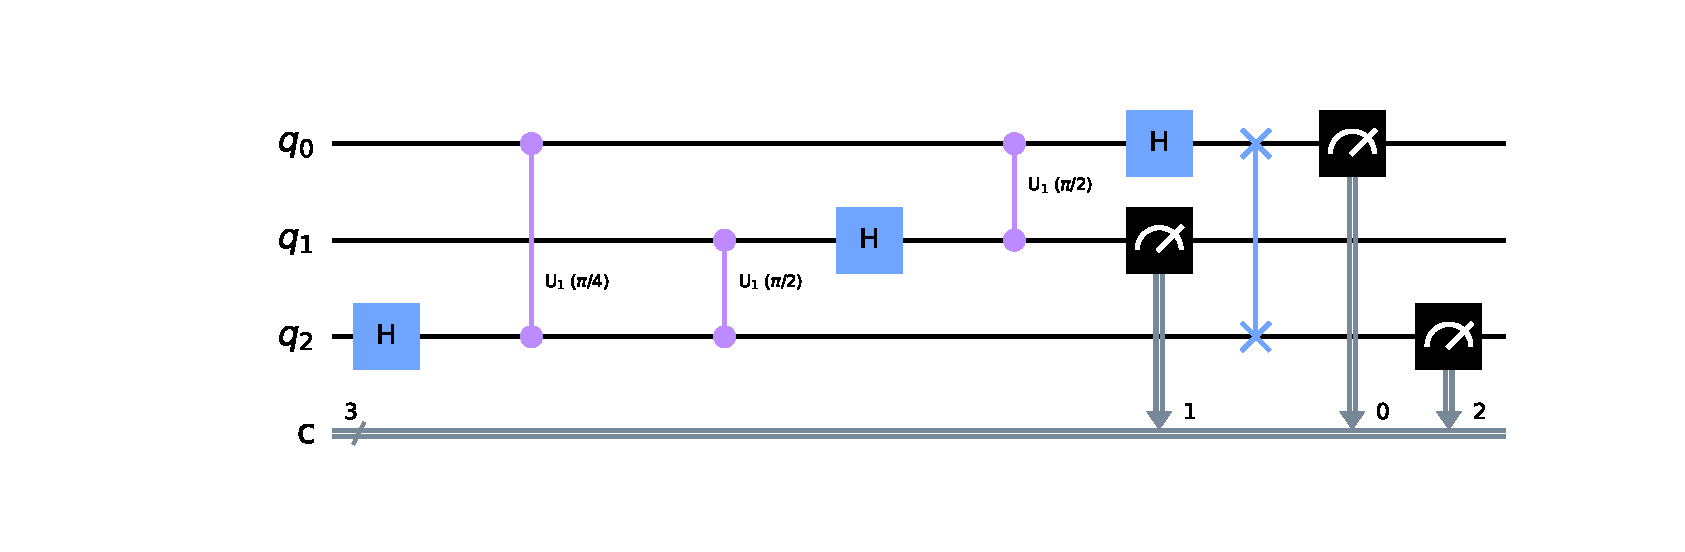
\includegraphics[width=0.86\textwidth]{qft.pdf}
	\caption{QFT量子电路图}
	\label{fig:qpe}
\end{figure}

\section{量子相位估计(QPE)}
给定一个酉矩阵 $U$ 与其特征向量 $|\psi\rangle$ 和特征值 $e^{2\pi i\theta}$, 该算法能找到 $\theta$\cite{23}, 这个算法主要就是利用量子傅立叶变换来做的, 下面是其量子电路示意图:
\begin{figure}[h]
	\centering
	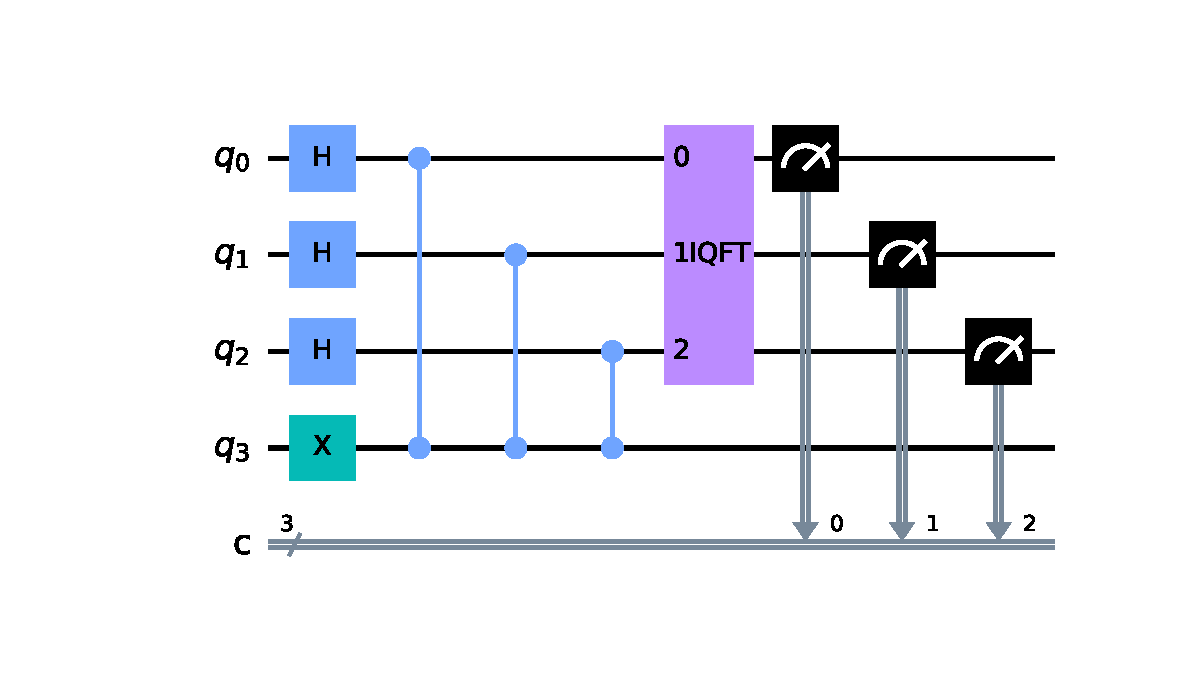
\includegraphics[width=0.7\textwidth]{qpe.pdf}
	\caption{QPE量子电路图}
	\label{fig:qpe}
\end{figure}




\chapter{量子算法求解线性方程组}

\section{HHL算法}
\subsection{算法简介}
要解决的问题:给定矩阵$A\in\mathbb{C}^{N\times N}$和向量$\vec{b}\in\mathbb{C}^{N}$, 找到$\vec{x}\in\mathbb{C}^{N}$, 满足$A\vec{x}=\vec{b}$.由于HHL算法\cite{16}\cite{24}是该领域最为经典的开山之作, 在此我详细的介绍一下这个算法.\par

使用量子计算机解决线性方程组的第一步是将问题编码为量子语言, 可以先假设 $\vec{b}$ 和 $\vec{x}$ 被单位化, 并将它们映射到相应的量子态 $|b\rangle$ 和 $|x\rangle$.通常, 可以很自然的这样来看: $\vec{b}$ (或 $\vec{x}$)的第 $i$ 个组成部分对应于量子态 $|b\rangle$ (或 $|x\rangle$)的第 $i$ 个基态的振幅.那可以转化成考虑这样的一个问题:

\begin{equation}
	A|x\rangle = |b\rangle ,
\end{equation}

首先可以假定 $A$ 是厄米特矩阵, 如果不是的话, 那么构造一个

\begin{equation}
	A=\left( \begin{array}{cc}
		0 & A^H \\
		A & 0 \\
	\end{array} \right),
\end{equation}
因此它有谱分解如下

\begin{equation}
	A=\sum_{j=0}^{N-1}\lambda_j|u_j\rangle\langle u_j|, \quad \lambda_j \in \mathbb{R}.
\end{equation}
其中 $|u_j\rangle$ 是 $A$ 的第 $j$ 个特征向量, 对应的特征值为 $\lambda_j$.并且, 

\begin{equation}
	A^{-1}=\sum_{j=0}^{N-1}\lambda_j^{-1}|u_j\rangle\langle u_j|,
\end{equation}
把右侧按照 $A$ 的特征向量展开

\begin{equation}
	|b\rangle = \sum_{j=0}^{N-1}b_j|u_j\rangle, \quad b_j \in \mathbb{C}.
\end{equation}
这样的话, 左右同时乘以$A^{-1}$, 就可以得到

\begin{equation}
	|x\rangle = A^{-1}|b\rangle = \sum_{j=0}^{N-1}\lambda_j^{-1}b_j|u_j\rangle.
\end{equation}

\subsection{算法实现}
\subsubsection{算法步骤}
1. 载入数据 $|b\rangle \in \mathbb{ C }^{N}$.即, 执行变换
$ |0\rangle _{n_{b}} \mapsto |b\rangle _{n_{b}} $.\par
2. 应用量子相位估计

对于 HHL使用 QPE, 其中 $U = e^{iAt}$, $A$ 是我们想要解决的系统对应的矩阵.在这种情况下, 

\begin{equation}
	e^{iAt} = \sum_{j=0}^{N-1}e^{i\lambda_{j}t}|u_{j}\rangle\langle u_{j}|.
\end{equation}

然后, 对于特征向量 $|u_{j}\rangle_{n_{b}}$, 其具有特征值 $e^{i\lambda_{j}t}$, QPE 将输出 $|\tilde{\lambda}_{j}\rangle_{n_{l}}|u_{j}\rangle_{n_{b}}$.其中 $\tilde{\lambda}_{j}$ 表示对 $\lambda_{j}t / 2\pi$ 的 $n_{l}$-位二进制近似.因此, 如果每个 $\lambda_{j}$ 可以用 $n_{l}$ 位精确表示, 
\begin{equation}
	\operatorname{QPE}(e^{iAt}, \sum_{j=0}^{N-1}b_{j}|0\rangle_{n_{l}}|u_{j}\rangle_{n_{b}}) = \sum_{j=0}^{N-1}b_{j}|\lambda_{j}\rangle_{n_{l}}|u_{j}\rangle_{n_{b}}
\end{equation}\par
3. 添加一个辅助量子位, 并根据 $|\lambda_{ j }\rangle$ 条件执行旋转, 
\begin{equation} 
	\sum_{j=0}^{N-1} b _ { j } |\lambda _ { j }\rangle_{n_{l}}|u_{j}\rangle_{n_{b}} \left( \sqrt { 1 - \frac { C^{2}  } { \lambda _ { j } ^ { 2 } } } |0\rangle + \frac { C } { \lambda _ { j } } |1\rangle \right).
\end{equation}
其中 $C$ 是一个归一化常数, 并且, 如上所述, 应小于最小特征值 $\lambda_{min}$ 的幅度, 即 $|C| < \lambda_{min}$.\par
4. 应用 QPE$^{\dagger}$.
\begin{equation}
	\sum_{j=0}^{N-1} b _ { j } |0\rangle_{n_{l}}|u_{j}\rangle_{n_{b}} \left( \sqrt { 1 - \frac {C^{2}  } { \lambda _ { j } ^ { 2 } } } |0\rangle + \frac { C } { \lambda _ { j } } |1\rangle \right) .
\end{equation}\par
5. 测量辅助量子位.如果结果是 $1$, 寄存器的后测量状态是
\begin{equation}
	\left( \sqrt { \frac { 1 } { \sum_{j=0}^{N-1} \left| b _ { j } \right| ^ { 2 } / \left| \lambda _ { j } \right| ^ { 2 } } } \right) \sum _{j=0}^{N-1} \frac{b _ { j }}{\lambda _ { j }} |0\rangle_{n_{l}}|u_{j}\rangle_{n_{b}}.
\end{equation}
这相当于归一化的解.\par
6. 应用一个可观测量 $M$ 来计算 $F(x):=\langle x|M|x\rangle$.

\subsubsection{实际应用中的非精确 QPE}

实际上, 应用 QPE 到初始态后, 寄存器的量子态是

\begin{equation}
	\sum_{j=0}^{N-1} b_{j} \left(\sum_{l=0}^{2^{n_{l}}-1}\alpha_{l|j}|l\rangle_{n_{l}}\right)|u_{j}\rangle_{n_{b}},
\end{equation}
其中
$$
\alpha_{l|j} = \frac{1}{2^{n_{l}}}\sum_{k=0}^{2^{n_{l}}-1}\left(e^{2\pi i\left(\frac{\lambda_{j}t}{2\pi}-\frac{l}{2^{n_{l}}}\right)}\right)^{k}.
$$

用 $\tilde{\lambda_{j}}$ 表示 $\lambda_{j}$ 的最佳 $n_{l}$-位近似, $1\leq j\leq N$.然后我们可以重新标记 $n_{l}$-寄存器, 使得 $\alpha_{l|j}$ 表示 $|l + \tilde{\lambda}_{j}\rangle_{n_{l}}$ 的振幅.所以, 

\begin{equation}
	\alpha_{l|j} := \frac{1}{2^{n_{l}}}\sum_{k=0}^{2^{n_{l}}-1}\left(e^{2\pi i\left(\frac{\lambda_{j}t}{2\pi}-\frac{l+\tilde{\lambda}_{j}}{2^{n_{l}}}\right)}\right)^{k}.
\end{equation}

如果每个 $\frac{\lambda_{j}t}{2\pi}$ 可以用 $n_{l}$ 位二进制位精确表示, 那么对于所有 $j$, $1\leq j\leq N$, 有 $\alpha_{0|j}=1$ 并且对于所有 $l\neq 0$, $\alpha_{l|j}=0$.仅在这种情况下, 我们才能写出 QPE 后寄存器的状态是

\begin{equation}
	\sum_{j=0}^{N-1} b_{j}|\lambda_{j}\rangle_{n_{l}}|u_{j}\rangle_{n_{b}}.
\end{equation}
否则, 如果且仅当 $\frac{\lambda_{j}t}{2\pi}\approx\frac{l+\tilde{\lambda}_{j}}{2^{n_{l}}}$ 时, $|\alpha_{l|j}|$ 较大, 寄存器的状态是
\begin{equation}
	\sum_{j=0}^{N-1}\sum_{l=0}^{2^{n_{l}}-1}\alpha_{l|j}b_{j}|l\rangle_{n_{l}}|u_{j}\rangle_{n_{b}}.
\end{equation}

\subsubsection{示例}
给定矩阵
$
A = \begin{pmatrix}
	1 & -\frac{1}{3} \\
	-\frac{1}{3} & 1
\end{pmatrix}
$
, 和向量
$
|b\rangle = \begin{pmatrix}
	1 \\
	0
\end{pmatrix}
$.
目标是找到满足$Ax = b$的解$x$.

我们将使用一个量子位$n_b=1$来表示向量$|b\rangle$(以及之后的解$|x\rangle$), 两个量子位$n_l=2$来存储矩阵$A$的特征值的二进制表示, 以及一个辅助量子位来存储条件旋转是否成功.

计算得到的特征值分别为
$
\lambda_1 = \frac{2}{3}, \quad \lambda_2 = \frac{4}{3}.
$

使用QPE输出$\lambda_j$的二进制近似, 设置
$
t = 2\pi \cdot \frac{3}{8},
$
这样QPE会得出
$
\frac{\lambda_1 t}{2\pi} = \frac{1}{4}, \quad \frac{\lambda_2 t}{2\pi} = \frac{1}{2},
$

对应的二进制表示分别是
$
|01\rangle_{n_l}, \quad |10\rangle_{n_l}.
$

矩阵$A$的特征向量分别是
$
|u_1\rangle = \frac{1}{\sqrt{2}}\begin{pmatrix}1 \\ -1\end{pmatrix}, \quad |u_2\rangle = \frac{1}{\sqrt{2}}\begin{pmatrix}1 \\ 1\end{pmatrix}.
$

我们可以将向量$|b\rangle$写成$A$的特征基中的形式
$
|b\rangle_{n_b} = \sum_{j=1}^{2}\frac{1}{\sqrt{2}}|u_j\rangle_{n_b}.
$

接下来, 我们按照HHL算法的步骤进行:

1. 状态准备很简单, 因为$|b\rangle=|0\rangle$.

2. 应用QPE后, 得到
$
\frac{1}{\sqrt{2}}|01\rangle|u_1\rangle + \frac{1}{\sqrt{2}}|10\rangle|u_2\rangle.
$

3. 使用$C=1/8$进行条件旋转.其中$C$要小于最小的特征值$\frac{1}{4}$, 因为算法中的一些步骤需要根据特征值的逆来执行旋转, 并且这个$C$的选取还尽可能大, 这样的话辅助量子位测量得到$|1\rangle$的概率就会更大, 这意味着算法成功找到解的概率也越大.
\begin{align}
	&\frac{1}{\sqrt{2}}|01\rangle|u_1\rangle\left( \sqrt{1 - \frac{(1/8)^2}{(1/4)^2}} |0\rangle + \frac{1/8}{1/4} |1\rangle \right) + \frac{1}{\sqrt{2}}|10\rangle|u_2\rangle\left( \sqrt{1 - \frac{(1/8)^2}{(1/2)^2}} |0\rangle + \frac{1/8}{1/2} |1\rangle \right)\\
	=
	&\frac{1}{\sqrt{2}}|01\rangle|u_1\rangle\left( \sqrt{1 - \frac{1}{4}} |0\rangle + \frac{1}{2} |1\rangle \right) + \frac{1}{\sqrt{2}}|10\rangle|u_2\rangle\left( \sqrt{1 - \frac{1}{16}} |0\rangle + \frac{1}{4} |1\rangle \right).
\end{align}

4. 在应用 QPE$^{\dagger}$之后, 量子计算机的状态为
$$
\frac{1}{\sqrt{2}}|00\rangle|u_{1}\rangle\left( \sqrt { 1 - \frac { 1  } {4 } } |0\rangle + \frac { 1 } { 2 } |1\rangle \right) + \frac{1}{\sqrt{2}}|00\rangle|u_{2}\rangle\left( \sqrt { 1 - \frac { 1  } {16 } } |0\rangle + \frac { 1 } { 4 } |1\rangle \right).
$$

5. 当辅助量子位测量结果为 $1$ 时, 状态变为
$$
\frac{\frac{1}{\sqrt{2}}|00\rangle|u_{1}\rangle\frac { 1 } { 2 } |1\rangle + \frac{1}{\sqrt{2}}|00\rangle|u_{2}\rangle\frac { 1 } { 4 } |1\rangle}{\sqrt{5/32}}.
$$
显然
$$
\frac{\frac{1}{2\sqrt{2}}|u_{1}\rangle+ \frac{1}{4\sqrt{2}}|u_{2}\rangle}{\sqrt{5/32}} = \frac{|x\rangle}{||x||}.
$$

6. 无需使用额外的门, 我们可以计算 $|x\rangle$ 的范数:它是上一步中测量到 $1$ 的辅助量子位的概率.
$$
P(|1\rangle) = \left(\frac{1}{2\sqrt{2}}\right)^{2} + \left(\frac{1}{4\sqrt{2}}\right)^{2} = \frac{5}{32} = ||x||^{2}.
$$


\begin{algorithm}[H]
	\caption{模拟HHL量子电路}
	\KwIn{线性方程组定义:矩阵$A = \begin{bmatrix} 1 & -\frac{1}{3} \\ -\frac{1}{3} & 1 \end{bmatrix}$, 向量$b = [1, 0]^T$}
	
	\BlankLine
	\tcc{使用HHL算法求解}
	调用HHL包(算法的具体步骤已经很清楚, 在此不再赘述)求解, 得到量子态$A$\;
	
	\tcc{从量子求解结果中提取和处理解向量}
	使用\texttt{Statevector}从$A$中提取解向量, 提取解向量的组成部分, 
	规范化解向量\;
	
	\BlankLine
	\tcc{使用经典算法求解}
	将向量$b$规范化后, 使用\texttt{NumPyLinearSolver}求解, 得到经典解\;
	
	\BlankLine
	\tcc{结果可视化}
	使用Matplotlib绘制量子电路和求解结果\;
	
	\KwOut{\\ HHL: [1.125 0.275] \\ normal: [1.125 0.275]}
	
\end{algorithm}



\begin{figure}[h]
	\centering
	\begin{minipage}{0.65\linewidth}
		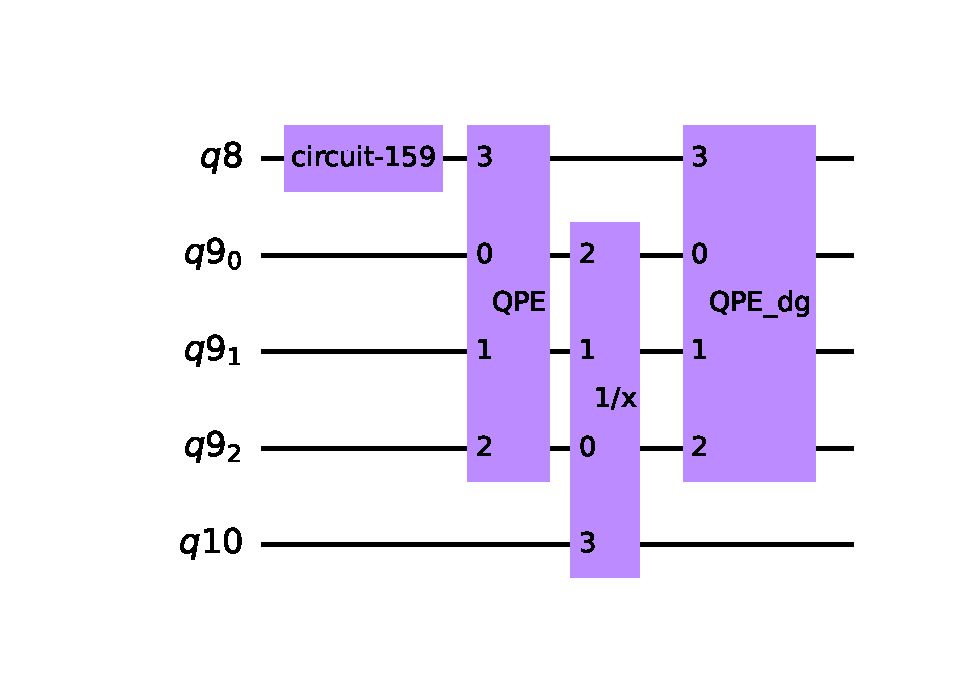
\includegraphics[width=\linewidth]{HHL.pdf}
		\caption{量子电路图}
	\end{minipage}
\end{figure}








\subsection{算法评估}
HHL算法对于特定类型的线性方程组, 提供了相对于经典算法的指数级加速算法的总体时间复杂度大致为 $O\left(\log(N) \kappa^2 / \epsilon\right)$, $\kappa$是矩阵$A$的条件数, $\epsilon$是算法的精度, 显然传统的方法在用时上完全不能和HHL算法相提评论, 因此这个方法对于处理大规模线性方程组还是有很大的价值的, 这展示了量子计算的强大优势和发展潜力.\par
相位估计这中需要$O(\log(N))$ 量子位进行编码, 复杂度为 $O\left(\kappa \log(N)/\epsilon\right)$, 由此可见, 这一算法还是很依赖矩阵的条件数的.并且, 因为需要高度控制的量子操作, 所以目前HHL算法的实际实现还是非常复杂的, 算法的实际执行会受到噪声的影响导致出现错误, 并且这个算法从设计上就只是得到量子态形式的解, 还需要额外的步骤才能得到我们所需要的具体数值.因此, 总得来看, 目前主要能够改进的算法还是在相位估计这一部分, 硬件方面相信随着量子纠错等领域的快速发展, 在未来正确率会越来越高, 逐渐的趋于实用.

\section{求解线性方程组的改进算法}
在HHL算法的基础上, 近十年以来, 科学家们为了降低算法的实际实现难度, 提高算法的效率和准确度, 提出了多种改进算法.其中, 变分量子算法是目前最为主流的研究方向.\par
变分量子线性求解器(Variational quantum linear solver)\cite{25}是一种利用变分原理来求解线性方程组的量子算法.该算法通过优化参数化的量子电路来最小化某个特定的成本函数, 从而找到线性方程组的解.

给定一个稀疏矩阵$M \in \mathbb{C}^{N\times N}$和一个初始状态向量$\ket{v_0}$, 想要计算规一化状态
\begin{align} 
	\ket{v_M} = \frac{M \ket{v_0}}{\|M \ket{v_0}\|},
\end{align}
其中$\|M \ket{v_0}\| = \bra{v_0}M^\dag M \ket{v_0}$且$M\ket{v_0}\ne 0$.\par 考虑$M$是非厄米特矩阵, 发现$\ket{v_M}$是哈密顿量
\begin{align}
	H_{M}=I-\frac{M\ket{v_0}\bra{v_0}{M^\dag}}{\|M \ket{v_0}\|^2},
\end{align}
的基态, 其能量为$0$.\par
使用真正的通用量子计算机, 可以应用常规技术, 如绝热态制备和相位估计等等来找到$H_{M}$的基态.不过, 对于NISQ设备, 要考虑使用参数化态的变分方法.\par
主要思想是首先考虑一个状态或ansätz\footnote[2]{是一个德语词汇, 在物理学、数学和相关领域中广泛使用, 尤其是在解决复杂方程和系统时.它指的是一个基于直觉、经验或理论预期的初始假设或有根据的猜测.这个假设通常用于简化问题, 为求解方程或系统提供一个出发点, 特别是在解析解或精确解难以直接获得的情况下.在量子计算和量子信息中, 通常指的是一个选择性的量子态或波函数形式, 用于近似描述系统的真实量子态.}, 
\begin{equation}
	\ket{\phi(\vec{\theta})}=U(\vec{\theta})\ket{0},
\end{equation}
其中$U(\vec{\theta}) = U_L(\theta_L)\dots U_2(\theta_2)U_1(\theta_1)$, $\vec{\theta}=(\theta_1,\theta_2,...,\theta_L)$.

\par 假设$H_{M}$的基态可以由ansätz在某些参数下表示, 那么寻找基态的问题就转化为最小化问题, 
\begin{align}
	\vec{\theta}_{\min}=\arg \min_{\vec{\theta}}\bra{\phi(\vec{\theta})} H_{M} \ket{\phi(\vec{\theta})}.
\end{align}
解由$\ket{v_M} = \ket{\phi(\vec{\theta}_{\min})}$给出. \par 最小化可以通过各种方法完成, 例如基于梯度的经典优化VQE、全局搜索算法、自适应变分算法、ITE等.以VQE为例, 我们从解的猜测$\vec{\theta}_0$开始, 并沿着能量$E_M(\vec\theta) = \bra{\phi(\vec{\theta})}H_{M}\ket{\phi(\vec{\theta})}$的负梯度更新参数, 
\begin{equation}
	\vec{\theta}_{i+1} = \vec{\theta}_{i} - a \nabla E_M(\vec\theta_i), \,\forall i  = 0, 1, \dots, T.
\end{equation}
其中$a$是时间步长, $T$是总步数.我们将在下一节展示如何测量梯度$\nabla E_{M}(\vec\theta_i)$.

接下来, 考虑求解线性方程组的问题.给定一个稀疏的$N \times N$矩阵$M$和一个初始状态向量$\ket{v_0}$, 我们想要计算
\begin{align} 
	\ket{v_{M^{-1}}} = \frac{M^{-1} \ket{v_0}}{\|M^{-1} \ket{v_0} \|},
\end{align}
其中状态通过$\|M^{-1} \ket{v_0} \| = \sqrt{\bra{v_0}({M}^{-1})^{\dagger} {M}^{-1} \ket{v_0}}$规范化, $M^{-1} \ket{v_0}\ne 0$.
\par 当矩阵$M$不是厄米特的时, 总是可以通过添加一个辅助量子比特将其转换为等效的厄米特矩阵问题.因此, 只需考虑$M$是厄米特且可逆的情况.解$\ket{v_{M^{-1}}}$是哈密顿量
$H_{M^{-1}}=M^\dag (I-\ket{v_0}\bra{v_0})M$
的基态, 其能量为$0$.在这里, 考虑以下优化问题
\begin{align}
	\vec{\theta}_{\min}=\arg \min_{\vec{\theta}}\bra{\phi(\vec{\theta})} H_{M^{-1}} \ket{\phi(\vec{\theta})},
\end{align}
其中$\ket{v_{M^{-1}}} = \ket{\phi(\vec{\theta}_{\min})}$.\par 使用VQE,从猜测$\vec{\theta}_0$开始, 并通过更新参数来降低哈密顿量的期望值$\bra{\phi(\vec{\theta})}H\ket{\phi(\vec{\theta})}$
\begin{equation}
	\vec{\theta}_{i+1} = \vec{\theta}_{i} - a \nabla E_{M^{-1}}(\vec\theta_i), \,\forall i  = 0, 1, \dots, T.
\end{equation}
其中能量$E_{M^{-1}}(\vec\theta) = \bra{\phi(\vec{\theta})}H_{M^{-1}}\ket{\phi(\vec{\theta})}$, 时间步长为$a$, 总步数为$T$.

通过这种方式, 算法试图找到能量的全局最小值对应的参数$\vec{\theta}{\min}$, 以及对应的量子态$\ket{\phi(\vec{\theta}{\min})}$, 这个量子态是我们希望得到的解.

VQLS算法相对于HHL算法而言, 更加适用于现阶段的NISQ设备, 因为它可以有效地减少量子操作的数量和复杂度, 从而降低错误率对算法准确性的影响.Adiabatic ansatz VQLS\cite{26}结合了绝热量子计算和变分量子算法的优点, 通过慢慢变化系统的哈密顿量, 使系统始终保持在基态附近, 从而避免了算法执行过程中的能级跃迁,这对于噪声的处理还是很有好处的.Evolutionary ansatz VQLS\cite{27}利用遗传算法来优化变分量子电路的结构和参数.通过自然选择、遗传等生物进化机制能够自动地发现和优化有效的量子电路, 以求解特定的线性方程组.Classical combination of quantum state(CQS)\cite{28}通过将线性方程组的解表示为多个量子态的线性组合, 然后利用经典优化算法来确定这些量子态前面的系数.这种方法的优势在于它充分利用了现有的量子硬件, 同时减少了量子操作的数量, 可以在目前不可避免的有噪声的环境下保持较高的求解精度. Logical ansatz VQLS\cite{29}是对CQS的一个改进, 它通过组合多个简单的变分量子电路来构建复杂的求解过程.每个简单电路负责捕捉线性方程组解的一部分特征, 通过逻辑组合这些简单电路能够有效地求解复杂的线性方程组.
\par
总的来看\cite{30}, VQLS方法和AAVQLS都表现出对量子设备上的噪声高度敏感, 引入实际设备的噪声水平之后, 两种方法性能都大幅度下降, 相比之下, EAVQLS则显示出更好的噪声抵抗能力.CQS是唯一一个真正使用量子计算机测试, 并且解决具有实际意义的问题的算法, 能够得到较为接近问题的真实解.LAVQLS在不引入噪声的情况下, 效果要优于CQS但是在引入噪声的情况下表现不佳.未来主要的发展方向还是应该好好的开发训练程序, 以避免AAVQLS之类的算法找不到基态而是误导成其它量子态.
\chapter{量子算法求解微分方程}
\section{量子算法求解ODE}
\begin{equation}\label{eqn:ODE_general}
	\left\{\begin{aligned}
		&\frac{d}{dt} u(t)= Au(t) + b(t), \quad t \in [0,T], \\
		&u(0) = u.
	\end{aligned}\right.
\end{equation}
其中 $u(t) \in \mathbb{C}^N$ 表示这个ODE的解, $A \in \mathbb{C}^{N\times N}$是系数矩阵,  $b(t) \in \mathbb{C}^N$ 是非齐次项. 
\subsection{算法理论的分析 }
考虑具有时间无关系数矩阵$A$和非齐次项$b$的常微分方程
\begin{equation}\label{eqn:ODE}
	\left\{\begin{aligned}
		&\frac{d}{dt} u(t)= Au(t) + b(t), \quad t \in [0,T], \\
		&u(0) = u.
	\end{aligned}\right.
\end{equation}

首先考虑齐次情况, 也就是\cref{eqn:ODE}中$b=0$的情况, 有以下几条定理\cite{31}.
\begin{theorem}\label{prop:lb_eig_diff_homo}
	给定一个可对角化矩阵$A = VDV^{-1}$, 其中$D = \text{diag}(\lambda_1,\cdots,\lambda_N)$是一个对角矩阵, $V$是一个可逆矩阵.假设$b = 0$.那么存在一个初始条件$u(0)$的实例, 对于\cref{eqn:ODE}, 任何量子算法输出$u(T)/\|u(T)\|$, 带有界定的错误和失败概率, 必须具有最坏情况下的查询复杂度$\Omega(e^{T\max_{i\neq j}|\text{Re}(\lambda_i-\lambda_j)|})$, 对$\ket{u(0)}$的准备oracle及其逆版本或控制版本.
\end{theorem}
\begin{theorem}\label{prop:lb_non_normal_homo}
	考虑线性ODE问题\cref{eqn:ODE}.让$\mu(A) = |A^{\dagger}A-AA^{\dagger}|^{1/2}$.然后存在\cref{eqn:ODE}的一个实例, 满足$b=0$, $A$是可对角化的并且所有特征值具有相等的实部, 这样任何量子算法输出$u(T)/|u(T)|$在有界误差和失败概率下, 必须具有最坏情况下的查询复杂度$\Omega(\mu(A))$到$\ket{u(0)}$的准备算符, 逆版本或控制版本.
\end{theorem}
现在考虑
\begin{equation}\label{eqn:ODE_ITE}
	\frac{d}{dt} u(t) = -H u(t), \quad t \in [0,T],
\end{equation}
其中$H$是一个半正定厄米特矩阵\cref{eqn:ODE_ITE}的解为
\begin{equation}
	u(T) = e^{-HT}u(0),
\end{equation}
虚时间演化问题就是准备量子态$e^{-HT}\ket{u(0)}/\xi$的近似, 其中$\xi = |e^{-HT}\ket{u(0)}|$.

\begin{theorem}
	如果$\xi = |e^{-HT}\ket{u(0)}|$, 那么存在\cref{eqn:ODE_ITE}的一个实例, 使得任何量子算法输出$u(T)/|u(T)|$在有界误差和失败概率下, 必须具有最坏情况下的查询复杂度$\Omega(1/\xi)$到$\ket{u(0)}$的准备算符, 逆版本或控制版本.
\end{theorem}
在非齐次情况下也有类似的结论:
\begin{theorem}\label{prop:lb_eig_diff_inhomo}
	给定一个可对角化矩阵$A = VDV^{-1}$, 其中$D = \text{diag}(\lambda_1,\cdots, \lambda_N)$是一个对角矩阵, $V$是一个可逆矩阵.那么存在向量$b$和初始条件$u(0)$的一个实例, 使得任何量子算法输出$u(T)/|u(T)|$在有界误差和失败概率下, 必须具有最坏情况下的查询复杂度$\Omega(e^{Y T}/(T+1+\sqrt{2}))$到$\ket{u(0)}$的准备算符, 逆版本或控制版本, 其中
	$Y = \min\left( \max_j \text{Re}(\lambda_j), \max_{i,j} \text{Re}(\lambda_i-\lambda_j) \right)$.
\end{theorem}

\begin{theorem}\label{prop:lb_non_normal_inhomo}
	考虑线性ODE问题\cref{eqn:ODE}.让$\mu(A) = |A^{\dagger}A-AA^{\dagger}|^{1/2}$.那么存在\cref{eqn:ODE}的一个实例, 使得任何量子算法输出$u(T)/|u(T)|$在有界误差和失败概率下, 必须具有最坏情况下的查询复杂度$\Omega(\mu(A))$到$\ket{u(0)}$的准备算符, 逆版本或控制版本.
\end{theorem}

\begin{theorem}[时间和精度的下界]
	\label{prop:lb_ND_inhomo}
	考虑线性ODE问题\cref{eqn:ODE}.让$l(A)$表示$A$的对数范数,定义为$(A+A^{\dagger})/2$的最大特征值.假设对于有$l(A) < 0$的线性方程系统$Ax = b$解决到误差$\epsilon$的最坏情况下量子查询下界是$\Omega(\log^{\alpha}(1/\epsilon))$,那么任何量子算法近似$u(T)/|u(T)|$到误差$\epsilon$必须具有最坏情况下的查询复杂度$\Omega(\min\left\{ \Omega\left(\log^{\alpha}(1/\epsilon)\right), \Omega\left(T^{\alpha}\right) \right\})$到相同的算符.
	
\end{theorem} \par
这一部分的定理通过证明最坏情况下的下界讨论了量子计算求解常微分方程的局限性, 表明了现有的量子算法可能再做很难改进.
\subsection{离散化时间的方法}
对于解决具有与时间无关的$A$和$b$的常微分方程(ODES), 最佳的通用算法基于泰勒展开\cite{32}, 而对于具有随时间变化的$b(t)$的ODE, 最佳方法是量子谱方法\cite{33}.这些方法的核心想法还是使用传统的方法先把ODE转化成线性方程组, 然后再使用上一章提到的各种方法再来求解线性方程组.

\begin{method}[\cite{32}]\label{lem:DEsolver_TI}
	考虑解决\cref{eqn:ODE_general}中的非齐次项$b$与时间无关.
	假设$A$是一个$N\times N$的$s$-稀疏矩阵\footnote[3]{在其每一行或每一列中, 至多只有s个非零元素.}, 具有稀疏输入预言机.对于$u(0)$和$b$, 我们假设它们的范数已知且给出了可以准备它们的预言机.那么存在一个量子算法, 以$2$-范数意义上的$\epsilon$-近似产生$u(T)/\|u(T)\|$, 成功概率为$\Omega(1)$, (也就是说存在一个常数$c>0$, 使得该事件的成功概率至少为$c$, 且这个常数$c$不依赖于问题的规模.)查询复杂度为
	\begin{equation}
		\widetilde{\mathcal{O}}\left( g T \|A\| C(A) \text{poly}\left(s,\log(N), \log\left(1+{Te^2\|b\|}/{\|u(T)\|}\right), \log(1/\epsilon)\right) \right),
	\end{equation}
	其中
	$$
	g = \frac{\sup_{t\in[0,T]}\|u(t)\| }{\|u(T)\|}, \quad C(A) = \sup_{t\in[0,T]} \|e^{At}\|. 
	$$
\end{method}

\begin{method}[\cite{33}]\label{lem:DEsolver_TD}
	考虑解决具有时间依赖的$b(t)$的~\cref{eqn:ODE_general}.
	假设$A$是一个$N\times N$的$s$-稀疏矩阵, 具有稀疏输入预言机, 并且可以对角化为$A = V\Lambda V^{-1}$, 其中$\Lambda = \text{diag}(\lambda_0,\cdots,\lambda_{N-1})$, 每个$j$的$\text{Re}(\lambda_j) \leq 0$.
	对于$u(0)$和$b(t)$, 我们假设它们的范数已知且给出了它们的准备预言机.
	那么存在一个量子算法, 以$2$-范数意义上的$\epsilon$-近似产生$u(T)/\|u(T)\|$, 成功概率为$\Omega(1)$, 查询复杂度为
	\begin{equation}
		\widetilde{\mathcal{O}}\left( g T \|A\| s \kappa_V \text{~poly}\log\left(\frac{ \max_{t\in[0,T],k \geq 1}\|u^{(k)}(t)\| }{\epsilon \|u(T)\|}\right) \right),
	\end{equation}
	其中
	$$
	g = \frac{\sup_{t\in[0,T]}\|u(t)\| }{\|u(T)\|}, \quad \kappa_V =\|V\|\|V^{-1}\|.  
	$$
\end{method}

在大多数现有基于解线性方程组的算法中, 对$A$和$u(0)$的准备预言机的查询数量的缩放在渐近上是相同的.然而, 最近的一项工作\cite{35}提出了一种用于解决齐次ODE的时间推进策略, 其中对准备预言机的查询数量在渐近上较小.
\begin{method}[\cite{34}]\label{lem:DEsolver_TM}
	考虑解决\cref{eqn:ODE_general}的齐次情况(即$b = 0$).
	假设$\|u(0)\| = 1$, 并且我们给定了矩阵$A$的$(\alpha,n_A,0)$-块编码 \cite{36}和$u(0)$的准备预言机.
	那么存在一个量子算法, 以$2$-范数意义上的$\epsilon$-近似产生$u(T)/\|u(T)\|$, 成功概率为$\Omega(1)$, 
	需要对$A$的块编码进行
	$$
	\widetilde{\mathcal{O}}\left( \alpha^2 T^2 Q \log(1/\epsilon) \right)
	$$
	次查询, 需要对$u(0)$的准备预言机进行
	$$
	\mathcal{O}\left( Q \right)
	$$
	次查询, 其中
	$$
	Q = \frac{\|e^{AT}\|}{\|u(T)\|}.
	$$
\end{method}

\subsection{非离散化时间的方法}
目前这方面没有通用的量子算法, 对于特定的ODE无需时间离散化和其余的运算, 下面我来介绍一个例子.

令$A \in \mathbb{C}^{N\times N}$为一个负定的厄米特矩阵.为了简化, 可以假设$\|A\| \leq 1$.假设我们有$A$的一个$(1,n_A,0)$-块编码的酉矩阵$U_A$.此外, 假设$O_u$和$O_b$是预言机, 使得$O_u \ket{0} = \frac{1}{\|u(0)\|} \sum_{j=0}^{N-1} u_j(0) \ket{j}$和$O_b \ket{0} = \frac{1}{\|b\|} \sum_{j=0}^{N-1} b_j \ket{j}$, 并假设$\|u(0)\|$和$\|b\|$是已知的.\par
考虑齐次情形, 获得二次加速的关键组件是指数函数$e^{-T(1-x)}$\cite{31}\cite{36}, 这可以被一个度为$\mathcal{O}(\sqrt{T})$的多项式近似, 并且可以使用QSVT\cite{36}实现.然后, 从$A$的块编码出发, 首先使用线性组合的幺正技术\cite{37}构造$(I+A)/2$的块编码, 然后通过均匀放大奇异值构造$(I+A)$的块编码\cite{36}.这里我们要求矩阵$A$是负定的以控制近似误差.然后, 算子$e^{AT} = e^{-T(I-(I+A))}$可以使用$e^{-T(1-x)}$的电路进行块编码, 查询复杂度为$\mathcal{O}(\sqrt{T})$.
\begin{theorem}
	考虑解决\cref{eqn:ODE}中$b = 0$且$A$是一个负定的厄米特矩阵, 使得$A$的所有特征值都在区间$[-1,-\delta]$内, 其中$\delta > 0$.假设我们给定了$A$的一个$(1,n_A,0)$-块编码, 记为$U_A$.那么对于任何$T>0$和$\epsilon<1/4$, 可以构造一个$(3,n_A+4,\epsilon)$-块编码的$e^{AT}$, 这需要使用
	\begin{equation}
		\mathcal{O}\left(  \frac{\sqrt{T}}{\delta}\log\left(\frac{1}{\epsilon}\right)\log\left(\frac{T\log(1/\epsilon)}{\epsilon}\right) \right)
	\end{equation}
	次查询,从而得到$U_A$逆版本和控制版本, 以及
	\begin{equation}
		\mathcal{O}\left(\left(n_A+\frac{1}{\delta}\log\left(\frac{T\log(1/\epsilon)}{\epsilon}\right)\right)\sqrt{T}\log\left(\frac{1}{\epsilon}\right) \right)
	\end{equation}
	个额外的1或2个量子门.
\end{theorem}

为了解决齐次ODE, 我们首先应用$O_u$准备$\ket{0}_a\ket{u(0)}_s$(其中“a”指古典辅助比特, “s”指状态寄存器), 然后应用$e^{AT}$的块编码得到$\ket{0}_a C \ket{\psi}_s + \ket{1}_a C' \ket{\psi'}_s$, 其中$C$是一个重缩放因子.这里$C \ket{\psi}_s$是$\frac{1}{3\|u(0)\|}e^{AT}u(0) = \frac{1}{3\|u(0)\|}u(T)$的$\mathcal{O}(\epsilon')$-近似.测量辅助比特并得到$0$产生$\mathcal{O}(\epsilon'\|u(0)\|/\|u(T)\|)$近似的$\ket{u(T)}$.我们选择$\epsilon' = \epsilon \|u(T)\|/\|u(0)\|$以限制错误在$\epsilon$以内.通过振幅放大, 成功概率可以提升到$\Omega(1)$, 通过重复过程$\mathcal{O}(\|u(0)\|/\|u(T)\|)$次.因此总体查询复杂度为
\begin{equation}
	\widetilde{\mathcal{O}}\left(\frac{\|u(0)\|}{\|u(T)\|} \frac{\sqrt{T}}{\delta}\log^2\left(\frac{1}{\epsilon}\right) \right). 
\end{equation}
\subsection{小结}
目前这些通过将时间和空间全部离散化之后再使用HHL算法以及其改进算法进行求解的量子算法, 对于ODE来说实际上量子优势还是比较微弱的, 这是由于目前HHL算法等还需要要求系数矩阵A是酉矩阵, 这就使得把一个常规的ODE离散化, 然后再通过提高维度的方法将系数矩阵变为酉矩阵, 这个过程是十分复杂并且也非常占用计算资源的.

\section{量子算法求解PDE}
\subsection{线性PDE}
目前在量子算法求解PDE这个问题上, 从现有的论文来看, 大体的研究思路还是和ODE一样, 使用传统的方法对时间和空间一起做离散化, 然后再使用量子算法来解线性方程组.不对时间离散化的方法也和上面的ODE相同, 通过快编码以及线性组合的玄正技术包括虚时间演化法(只能做热方程)\cite{38}等等.\par 近期还有薛定谔化方法\cite{39}, 这种方法相比于其它的办法来说更加自然一些, 可以通过提高维度来将全部的ODE和PDE转化成薛定谔方程, 这是一个非常好的思路.\par 以热方程为例:
\begin{equation}
	\left\{\begin{array}{l}
		\partial_t u-\Delta u=0, \\
		u(0, x)=u_0(x).
	\end{array}\right.
\end{equation}
\begin{center}
	$u=u(t, x), \quad x=\left(x_1, x_2, \cdots, x_d\right) \in \mathbb{R}^d$ , \quad  $t \geq 0$.
\end{center}
引入一个新的变量 $p>0$ , 定义
\begin{equation}
	w(t, x, p)=\mathrm{e}^{-p} u(t, x), \quad p>0 .
\end{equation}
原方程可以转化为
\begin{equation}\label{2}
	\partial_t w+\partial_p \Delta_x w=0, \quad p>0 ;
\end{equation}
从$w$转化回$u$可以通过
\begin{equation}
	u(t, x)=\int_0^{\infty} w(t, x, p) \mathrm{d} p \quad \text { 或者 } \quad u(t, x)=\mathrm{e}^{p_*} w\left(t, x, p_*\right) , \text { 任取 } p_*>0
\end{equation}

对于\cref{2}中的$x$做Fourier变换得到 
\begin{equation}
	\partial_t \hat{w}-|\xi|^2 \partial_p \hat{w}=0.
\end{equation}

这是一个对流方程, 并且是一个从右边往左边传的波, 所以选一个足够大的$p$就可以作为右边的b边值条件, 而左边$p$是0, 因此通过升维得到的是一个适定的PDE.
接下来, 为了便于对$p$做Fourier变换, 可以将$p$延拓到全空间上, 
\begin{equation}
	\left\{\begin{array}{l}
		\partial_t w+\Delta_x \partial_p w=0, \quad p \in(-\infty, \infty), \\
		w(0, x, p)=\mathrm{e}^{-|p|} u_0(x) .
	\end{array}\right.
\end{equation}

对 $p$ 做Fourier变换, 可以得到
\begin{equation}
	\mathrm{i} \partial_t \tilde{w}=\eta \Delta \tilde{w}, 
\end{equation}
这便得到了薛定谔方程.

不止如此, 这个方法对于ODE也同样适用的, 下面是一个一般的例子
\begin{equation}
	\left\{\begin{array}{l}
		\frac{\mathrm{d} \boldsymbol{u}(t)}{\mathrm{d} t}=A \boldsymbol{u}(t) ,\\
		\boldsymbol{u}(0)=\boldsymbol{u}_0.
	\end{array} \quad A^{\dagger} \neq A.\right.
\end{equation}
让
\begin{equation}
	A=H_1+\mathrm{i} H_2 , H_1=\frac{A+A^{\dagger}}{2}=H_1^{\dagger},  H_2=\frac{A-A^{\dagger}}{2 \mathrm{i}}=H_2^{\dagger} .
\end{equation}
这是容易做到的, 接下来还是引入$\mathrm{e}^{-p}$, 
\begin{equation}
	\boldsymbol{v}(t, p)=\mathrm{e}^{-p} \boldsymbol{u}(t) ,  p>0;
\end{equation}

\begin{equation}
	\left\{\begin{array}{l}
		\frac{\mathrm{d}}{\mathrm{d} t} \boldsymbol{v}(t, p)=A \boldsymbol{v}(t, p)=-H_1 \partial_p \boldsymbol{v}+\mathrm{i} H_2 \boldsymbol{v} ,\\
		\boldsymbol{v}(0, p)=\mathrm{e}^{-|p|} \boldsymbol{u}_0 .
	\end{array}\right.
\end{equation}

关于$p$做离散傅里叶变换可以得到
\begin{equation}
	\begin{aligned}
		&\tilde{\boldsymbol{w}}=\left(I_u \otimes F_n^{-1}\right) \boldsymbol{w} ;\\
		&D_\mu=\operatorname{diag}\left(\mu_1, \cdots, \mu_M\right); \\
		&\frac{\mathrm{d}}{\mathrm{d} t} \tilde{\boldsymbol{w}}(t)=-\mathrm{i}\left(H_1 \otimes D_\mu\right) \tilde{\boldsymbol{w}}+\mathrm{i}\left(H_2 \otimes I\right) \tilde{\boldsymbol{w}} .
	\end{aligned}
\end{equation}

根据\cite{40}可知, 这个方法对于其它的线性PDE和ODE也同样适用, 例如线性Black-Scholes方程, Fokker-Planck方程, Maxwell方程组等等, 这是一个很好的研究方向.
\subsection{非线性PDE}
量子计算机本质上是一个物理设备, 因此它的行为一定也会遵循物理定律, 然而薛定谔方程是线性的, 因此从原理上来说, 量子计算机很难解决非线性的问题\cite{41}.然而目前很多重要的问题还是会涉及到非线性微分方程, 像流体运动的Navier-Stokes方程, 孤立波理论中的Korteweg-de Vries方程, 大气对流的Lorenz方程, 生物中的 Fisher方程和反应扩散方程等等.\par
如何求解非线性微分方程也是目前的一个很重要的研究方向, 由于很难发现基于新原理的计算机, 因此工作的重点还是在如何将非线性方程转化成线性的, 目前主要是线性近似, 以及直接寻找非线性方程的线性表示这两种思路.
\subsubsection{线性近似}
这种思路是将非线性项线性化, 不过这种线性近似的办法会丢失部分非线性特征丢失, 使得所描述的物理过程发生改变.
\begin{method}
	\cite{42}的主要原理是非线性薛定谔方程可以通过多个相同的相互作用的副本来模拟, 这些副本是遵循线性薛定谔方程的.设 $x \in {\cal C}^d$ 为一个 $d$ 维复向量空间中的状态向量.考虑以下形式的方程
	\begin{equation}
		\frac{dx}{dt} + f(x) x = b(t), \label{proximity}
	\end{equation}
	其中 $f(x)$ 是一个 $d \times d$ 矩阵, 它是向量 $x$ 和 $x^\dagger$ 的 $m$ 阶多项式函数.可以通过把 $x$ 的维度提高1维来把$f(x)$写成
	\begin{equation}
		f(x) = {x^\dagger}^{\otimes m} F x^{\otimes m}, 
	\end{equation}
	其中$F$是一个合适的张量 . 
	
	在这里考虑的应用中, 需要假设 $F$ 是稀疏的, 因此适用于那些由局部相互作用主导的物理系统描述的非线性方程.
	
	
	当 $f$ 是反厄米特矩阵, 并且 $b(t)=0$ 时, 基本方法如下.取初始状态 $x(0)^{\otimes n }$ 的 $n>>m$ 份副本(显然, 这个准备过程可能是相当困难的), 并对初始状态 $x(0)^{\otimes n }$ 应用哈密顿量
	\begin{equation}
		H = -i {n \choose m}^{-1} \sum_{j_1\ldots j_m} F_{j_1 \ldots j_m}, 
	\end{equation}
	这里 $F_{j_1\ldots j_m}$ 是应用于由 $j_1 \ldots j_m$ 标记的 $m$ 个不同子系统的张量 $F$.
	
	观察 $n$-系统线性薛定谔方程的短时间行为:
	\begin{equation}
		e^{-iH\Delta t} x^{\otimes n} = (I - iH\Delta t - \frac{1}{2} H^2 \Delta t^2 + O(\Delta t^3) ) x^{\otimes n}.
	\end{equation}
	通过追踪出其他副本, 可以获得任一副本的短时间行为, 从而得到单个系统的有效动力学行为:
	\begin{equation}
		x \rightarrow ( I -  \Delta t f(x)) x + O(E^2\Delta t^2), 
	\end{equation}
	其中 $E$ 是该时间段内 $|f(x)|$ 的平均值.
	
	在短时间内每个副本的行为与真实的、理想的非线性系统行为之间还是存在$1/n$量级的偏差, 其中$n$ 代表副本的数量, 并且如果只看方程中的一阶项, 这些偏差可能不是很明显;但当考虑到更二阶及以上时, 偏差就会被放大.
	
\end{method}
\begin{method}
	\cite{43}主要解决的是可以用二次多项式表示的耗散非线性微分方程, 由于耗散所以非线性效应只会在有限的时间内比较显著, 该方法考虑的就是在非线性效应没那么显著的时刻开始所做的线性近似.使用卡尔曼线性化方法, 将有限维非线性微分方程转化成无限维线性微分方程, 然后再根据近似误差的要求截断为有限维的.
	
	考虑由 $n$ 维二次常微分方程 (ODE) 描述的初值问题
	\begin{equation}
		\frac{\mathrm{d}u}{\mathrm{d}t} = F_2 u^{\otimes 2} + F_1 u + F_0(t), \qquad
		u(0) = u_{\mathrm{in}}.
		\label{eq:NODE}
	\end{equation}
	其中 $u=[u_1, \ldots, u_n]^{T}\in\mathbb{R}^n$, $u^{\otimes 2}=[u_1^2, u_1u_2, \ldots, u_1u_n, u_2u_1, \ldots, u_nu_{n-1}, u_n^2]^{T}\in\mathbb{R}^{n^2}$, 每个 $u_j = u_j(t)$ 是时间间隔 $[0,T]$ 上的 $t$ 函数, 对于 $j\in\{1,\ldots,n\}$, $F_2\in\mathbb{R}^{n\times n^2}$, $F_1\in\mathbb{R}^{n\times n}$ 是与时间无关的矩阵, 而非齐次项 $F_0(t)\in\mathbb{R}^n$ 是 $t$ 的 $C^1$ 连续函数. $\|\cdot\|$ 表示谱范数.
	
	考虑的主要计算问题如下.给定系统的二次常微分方程 \cref{eq:NODE}, 应用 Carleman 线性化程序得到线性常微分方程组
	\begin{equation}
		\frac{\mathrm{d}\hat y}{\mathrm{d}t} = A(t) \hat y + b(t), \qquad
		\hat y(0) = \hat y_{\mathrm{in}}.
		\label{eq:LODE}
	\end{equation}
	具有三对角块结构
	\begin{equation}
		\frac{\mathrm{d}}{\mathrm{d}t}
		\begin{pmatrix}
			\hat y_1 \\
			\hat y_2 \\
			\hat y_3 \\
			\vdots \\
			\hat y_{N-1} \\
			\hat y_N \\
		\end{pmatrix}
		=
		\begin{pmatrix}
			A_1^1 & A_2^1 &  &  &  &  \\
			A_1^2 & A_2^2 & A_3^2 & &  &  \\
			& A_2^3 & A_3^3 & A_4^3 &  &  \\
			&  & \ddots & \ddots & \ddots &  \\
			&  &  & A_{N-2}^{N-1} & A_{N-1}^{N-1} & A_N^{N-1} \\
			&  &  &  & A_{N-1}^N & A_N^N \\
		\end{pmatrix}
		\begin{pmatrix}
			\hat y_1 \\
			\hat y_2 \\
			\hat y_3 \\
			\vdots \\
			\hat y_{N-1} \\
			\hat y_N \\
		\end{pmatrix}+
		\begin{pmatrix}
			F_0(t) \\
			0 \\
			0 \\
			\vdots \\
			0 \\
			0 \\
		\end{pmatrix},
		\label{eq:UODE}
	\end{equation}
	其中 $\hat y_j=u^{\otimes j}\in\mathbb{R}^{n^j}$, $\hat y_{\mathrm{in}}=[u_{\mathrm{in}}; u_{\mathrm{in}}^{\otimes 2}; \ldots; u_{\mathrm{in}}^{\otimes N}]$, 和 $A_{j+1}^j \in \mathbb{R}^{n^j\times n^{j+1}}$, $A_j^j \in \mathbb{R}^{n^j\times n^j}$, $A_{j-1}^j \in \mathbb{R}^{n^j\times n^{j-1}}$ 对于 $j\in\{1,\ldots,N\}$ 满足
	
	\begin{align}
		A_{j+1}^j &= F_2\otimes I^{\otimes j-1}+I\otimes F_2\otimes I^{\otimes j-2}+\cdots+I^{\otimes j-1}\otimes F_2, \\
		A_j^j &= F_1\otimes I^{\otimes j-1}+I\otimes F_1\otimes I^{\otimes j-2}+\cdots+I^{\otimes j-1}\otimes F_1, \\
		A_{j-1}^j &= F_0(t)\otimes I^{\otimes j-1}+I\otimes F_0(t)\otimes I^{\otimes j-2}+\cdots+I^{\otimes j-1}\otimes F_0(t).
	\end{align}
	
	注意 $A$ 是一个 $(3Ns)$-稀疏矩阵.方程 \cref{eq:LODE} 的维度为
	$$
	n+n^2+\cdots+n^N=\frac{n^{N+1}-n}{n-1}=O(n^N).
	$$		
	为了构造线性方程组, 我们首先将时间区间 $[0,T]$ 划分为 $m = T/h$ 个时间步长, 并在方程 \cref{eq:LODE} 上应用向前欧拉法, 即
	\begin{equation}
		y^{k+1} = [I+A(kh)h] y^k + b(kh),
		\label{eq:forward}
	\end{equation}
	其中 $y^k \in \mathbb{R}^{\Delta}$ 近似于每个 $k \in \{0,1,\ldots,m\}$ 时刻的 $\hat y(kh)$, 初始值 $y^0 = y_{\mathrm{in}} \coloneqq \hat y(0) = \hat y_{\mathrm{in}}$, 并假设对于某个足够大的整数 $p$, 所有的 $y^k$ 对于 $k\in\{m+1,\ldots,m+p+1\}\setminus\{0,1,\ldots,m\}$ 都相等.
	
	这产生了一个 $(m+p+1)\Delta\times(m+p+1)\Delta$ 的线性系统
	\begin{equation}
		L|Y\rangle=|B\rangle,
		\label{eq:linear_system}
	\end{equation}
	该系统编码了方程 \cref{eq:forward} 并用于生成时间 $T$ 的数值解, 其中
	\begin{equation}
		L = \sum_{k=0}^{m+p}|k\rangle\langle k|\otimes I-\sum_{k=1}^{m}|k\rangle\langle k-1|\otimes [I+A((k-1)h)h]-\sum_{h=m+1}^{m+p}|k\rangle\langle k-1|\otimes I,
		\label{eq:matrixL}
	\end{equation}
	
	\begin{equation}
		|B\rangle = \frac{1}{\sqrt{B_m}}\Bigl(\|y_{\mathrm{in}}\||0\rangle \otimes |y_{\mathrm{in}}\rangle+\sum_{k=1}^{m}\|b((k-1)h)\||k\rangle \otimes |b((k-1)h)\rangle\Bigr),
		\label{eq:vectorB}
	\end{equation}
	其中 $B_m$ 是一个归一化因子.观察到系统 \cref{eq:linear_system} 有下三角结构.
	\begin{equation}
		\begin{pmatrix}
			I &  &  &  &  &  &  \\
			-[I\!+\!A(0)h] & I &  &  &  &  &  \\
			& \ddots & \ddots &  &  &  & \\
			&  & -[I\!+\!A((m-1)h)h] & I &  &  &  \\
			&  &  & -I & I &  &  \\
			&  &  &  & \ddots & \ddots & \\
			&  &  &  &  & -I & I \\
		\end{pmatrix}
		\begin{pmatrix}
			y^0 \\
			y^1 \\
			\vdots \\
			y^m \\
			y^{m+1} \\
			\vdots \\
			y^{m+p} \\
		\end{pmatrix}
		=
		\begin{pmatrix}
			y_{\mathrm{in}} \\
			b(0) \\
			\vdots \\
			b((m-1)h) \\
			0 \\
			\vdots \\
			0 \\
		\end{pmatrix}.
	\end{equation}
	
	在上述系统中, 对于 $k\in\{0,1,\ldots,m+p+1\}$, $y^k$ 的前 $n$ 个分即( $y_1^k$)归一化处理后近似于精确解 $u(T)$.我们应用QLSA到方程 \cref{eq:linear_system} 上, 并在 $k$ 上进行后选择, 以产生某个 $k\in\{m+1,\ldots,m+p+1\}\setminus\{0,1,\ldots,m\}$ 的 $y_1^k/\|y^k_1\|$.所得的误差最多为
	\begin{equation}
		\epsilon \coloneqq \max_{k\in\{m+1,\ldots,m+p+1\}\setminus\{0,1,\ldots,m\}}\left\|\frac{u(T)}{\|u(T)\|}-\frac{y^k_1}{\|y^k_1\|}\right\|.
		\label{eq:error}
	\end{equation}
	误差来自 Carleman 线性化和向前欧拉法.(QLSA 也会引入误差, 将单独限定.)\par
	对于这个算法而言, 系统必须是耗散的, 并且非线性和非齐次效应相对于线性效应必须是小的.
	并且在应用中, 这个方法产生了一个编码解决方案的状态向量, 而没有指定如何从该状态中提取信息.仅仅产生一个状态向量对于端到端的应用来说是不够的, 因为完整的量子状态不能高效地读取.在某些情况下, 通过采样一个简单的可观测量可能可以提取有用的信息, 而在其他情况下, 可能需要更复杂的后处理来推断解决方案的所需属性.这是该算法实际应用中的问题.
	
	
	
	
\end{method}
\subsubsection{直接线性表示}
该方法主要适用于非线性哈密顿-雅可比以及双曲方程\cite{44}.哈密顿-雅可比方程或非线性双曲方程的一个显著特点是, 即使初始数据是光滑的, 解也可能变得奇异.对于非线性双曲方程, 解可能会变得不连续, 而对于哈密顿-雅可比方程, 解可能形成尖点.当解变得奇异时, 由于导数项不再良定义, 需要对方程进行解释.在这方面, 人们要么使用粘性解的概念, 这在气体动力学中的压缩欧拉方程等应用中是物理上相关的, 要么使用哈密顿-雅可比-贝尔曼方程进行最优控制.另一个概念是多值解, 这与半经典量子动力学和几何光学等应用相关, 在这些应用中, 动力学是时间不可逆的, 解满足线性叠加原理.当解是光滑的, 这两个概念定义了相同的解, 但在奇点出现时则不然.在本文中, 以非线性哈密顿-雅可比为例, 讲述一下这个方法.\par

哈密顿-雅可比方程在几何光学、薛定谔方程的半经典极限、前沿传播的水平集公式化、最优控制、平均场游戏、无压气体或KPZ方程中出现.它具有以下一般形式
\begin{align}
	& \partial_t S^{[k]}+ H(\nabla S^{[k]}, x) = 0, \quad t\in \mathbb{R}^+,  x \in \mathbb{R}^d, S^{[k]}(t,x)\in \mathbb{R}, \label{H-J}\\
	&S^{[k]}(0,x)=S_0^{[k]}(x), \quad k=1,...,M.
\end{align}
其中对于每个$k$, 都满足相同的哈密顿-雅可比PDE, 即考虑$M$个不同的初始数据.

直接数值近似\cref{H-J}通常会导致所谓的粘性解.这种解的概念在很多物理过程中中不成立, 因为它违反了线性叠加原理, 因此人们感兴趣的是计算多值解, 这是目前相关的几种方法:\par
1. 射线追踪 \cite{45}.这是基于解决系统的特性, 即哈密顿系统
\begin{equation}\label{H-S}
	\partial_t x(t) = \nabla_p H(x,p)\,, \quad
	\partial_t p(t) = -\nabla_x H(x,p)\,.
\end{equation}
这种方法比较简单, 因为它只解决一组常微分方程.缺点是粒子分布不均匀, 可能会出现没有足够粒子以保证数值精度的区域, 需要添加更多粒子, 然后使用插值来定义这些粒子, 这是不好控制的.\par

2. 矩方法 \cite{46}.对于多值解, 可以使用矩系统, 这是哈密顿-雅可比方程的叠加.这种方法的优点是保持在物理空间中, 然而, 矩系统在高维中很难导出, 并需要预先知道分支的数量, 例如, 在光学中, 由于折射或反射, 光线可能沿着多个路径传播;在动力学系统中, 系统可能演化为几个不同的稳定状态;在解偏微分方程时, 尤其是涉及到非线性方程或具有复杂边界条件的情况, 可能会出现多个解.当使用矩方法处理这类问题时, 每个分支可能对应于解的一个不同的“矩”或统计特征.在实际使用中, 这几乎是一项不可能的任务.\par

3.  水平集法\cite{47}.在这里, 将$S$的梯度构建到解决一组刘维尔方程的函数的零水平集中 .这种方法全局有效, 可以得到一个线性的PDE系统.因为方程在相空间中定义, 维数加倍, 因此传统计算机很难使用, 不过这一点恰恰适合量子计算机. \\

定义$u^{[k]}=\nabla S^{[k]} \in \mathbb{R}^d$.然后$u^{[k]}$解决一个在梯度形式下的双曲系统保守律:
\begin{align}
	& \partial_t u^{[k]} + \nabla H(u^{[k]}, x) = 0, \label{forced-Burgers} \\
	&u^{[k]}(0,x)=\nabla S^{[k]}_0(x).
\end{align}


水平集函数$\phi^{[k]}_i(t,x,p)$可以通过以下方式定义
\begin{equation}
	\phi^{[k]}_i(t, x,p=u^{[k]}(t,x))=0.
\end{equation}
其中$i=1, \cdots, d$且$x, p\in \mathbb{R}^d$, $k=1,...,M$.

而$\{u^{[k]}(t,x)\}$是具有$M$个初始条件的非线性哈密顿-雅可比方程在梯度形式下的解, 见方程~\cref{forced-Burgers}. $\phi^{[k]}_i$的零水平集是集合$\{(t,x,p)|\phi^{[k]}_i(t,x,p)=0\}$.

由于$u^{[k]}(t,x)$是方程\cref{forced-Burgers}的解, 因此可以证明$\phi^{[k]}=(\phi^{[k]}_1, \cdots, \phi^{[k]}_d)\in \mathbb{R}^d$解决了一个线性的刘维尔方程
\begin{equation}
	\partial_t \phi^{[k]} + \nabla_p H \cdot \nabla_x \phi^{[k]} - \nabla_x H \cdot \nabla_p \phi^{[k]}=0.\label{LS-Liouville}
\end{equation}

注意到, 在刘维尔方程\cref{LS-Liouville}中, 方程的解沿着由方程\cref{H-S}定义的哈密顿系统的轨迹(或称为双特征线)演化.因此, 我们可以通过选择合适的初始数据来追踪这些解的行为.在这里, 初始数据可以选择为
\begin{equation}
	\phi^{[k]}_i(0, x,p)=p_i - u^{[k]}_i(0,x), \quad i=1, \cdots, d.
\end{equation}

然后, $u^{[k]}$可以从$\phi_i \, (i=1, \cdots, d)$的零水平集的交集中恢复, 如\cref{intersect}所示, 即
\begin{equation}
	u^{[k]}(t,x)=\{p(t,x)| \,\phi_i^{[k]}(t,x,p)=0, \, i=1,\cdots, d \}. 
\end{equation}

注意到, $\phi_i^{[k]}(t,x,p)=0$可能有多个(比如说$J_k$个根, 记为$p_{Y(t,x)} (Y=1, \cdots, J_k)$), 因此将出现多值解, 记为
\begin{equation}
	u^{[k]}_{Y}(t,x)= \cap_{i=1}^d \{p_{Y}(t,x) | \phi^{[k]}_i(t,x,p_{Y})=0\}, \quad Y=1, \cdots, J_k.\label{intersect}
\end{equation}

这样就可以将一个$(d+1)$维的非线性PDE——哈密顿-雅可比方程——转化为了一个$(2d+1)$维的线性PDE——刘维尔方程, 而没有对原始非线性的形式或范围做任何假设.并没有进行线性近似, 而是一个精确的映射.从非线性系统到线性系统的转换仅以增加维度为代价.之后可以将这个方程离散化, 使用HHL等算法求解方程组.








\chapter{结论}
量子计算展现出了巨大的潜力, 特别是在求解线性方程组的方面, HHL算法及其改进为传统计算机难以求解的高维度问题提供了新的路径.然而, 目前的量子算法大多仍处于理论阶段, 或者是模拟阶段, 并没有真正投入到量子计算机上去使用.并且, 量子计算机在硬件上也面临着许多挑战, 如量子比特的稳定性和噪声影响等, 这在短时间内还是难以攻克的.所以在未来还是应该着重发展如何克服噪声的影响的算法, 以及成本较低的量子纠错, 结合传统的方法, 开发出适合目前量子计算机的算法.

对于线性微分方程的求解, 量子算法同样展现出了强大的发展潜力, 不过目前大多数方法依赖于使用传统方法对原问题进行离散化, 然后再使用量子算法对得到的线性方程组进行求解.对于非线性问题, 目前也还缺少一种更加具有普适性的方法将其转化为非线性问题, 这是一个很重要的课题.我认为在未来, 研究重点可能会更多地放在开发不需要时间离散化的算法上, 以及如何有效地结合量子和经典算法来克服目前的硬件限制, 从而真正的发挥量子优势.或许通用量子计算机还很遥远, 但是可以根据特定的算法开发专门的量子模拟器, 从而解决特定的问题.